\section{Metasezgisel Optimizasyon Algoritmaları II}
Metasezgisel algoritmaların daha ileri uygulamaları ve hibrit yaklaşımlar bu bölümde incelenecektir. Modern optimizasyon problemlerinin çözümünde kullanılan gelişmiş teknikler ve bunların uygulamaları ele alınacaktır.

\subsection{Tavlama Benzetimi (Simulated Annealing) }
Tavlama Benzetimi (Simulated Annealing), metalurjideki tavlama işleminden esinlenen güçlü bir metasezgisel optimizasyon algoritmasıdır. Metallerin tavlama sürecinde, malzeme önce yüksek sıcaklıklara ısıtılır, bu sırada atomlar yüksek enerji seviyelerinde rastgele hareket eder. Ardından malzeme kontrollü bir şekilde yavaşça soğutulur, böylece atomlar düşük enerjili, kararlı bir kristal yapıya yerleşir. Bu fiziksel süreç, optimizasyon problemlerinde global optimuma ulaşmak için etkili bir strateji olarak uyarlanmıştır. Algoritma, başlangıçta yüksek "sıcaklık" parametresiyle çalışarak kötü çözümleri bile belirli bir olasılıkla kabul eder ve böylece geniş bir arama uzayını keşfeder. Sıcaklık kademeli olarak düştükçe, algoritma daha seçici hale gelir ve umut vadeden bölgelerde daha yoğun arama yapar. Bu yaklaşım, lokal optimumlara takılma riskini azaltarak, karmaşık ve çok modlu optimizasyon problemlerinde global optimuma yakınsama olasılığını artırır. \sidenote{Tavlama benzetimi, özellikle kombinatoryal optimizasyon problemlerinde başarılı sonuçlar verir. Sıcaklık düşüş hızı ve başlangıç sıcaklığı algoritmanın performansını etkileyen önemli parametrelerdir. Tavlama benzetimi algoritması kullanarak Ackley fonksiyonu üzerinde gerçekleştirilen örnek python kodu:

\qrcode[height=1in]{https://github.com/btayfur/structural-optimization/blob/main/Code/Examples/Exmp1}}

\subsubsection{Algoritmanın Temeli}
Metallerin tavlama işleminden esinlenmiş bir optimizasyon algoritması:
\begin{itemize}
    \item Yüksek sıcaklıkta rastgele hareketler
    \item Sıcaklık düştükçe kontrollü hareketler
    \item Kötü çözümlerin kabul edilme olasılığı
\end{itemize}

\begin{equation}
P(\Delta E) = \exp\left(-\frac{\Delta E}{kT}\right)
\end{equation}

\begin{figure}[h]
\centering
\begin{tikzpicture}
\draw[->] (0,0) -- (4,0) node[right] {İterasyon};
\draw[->] (0,0) -- (0,4) node[above] {Sıcaklık};
\draw[scale=1,domain=0:4,smooth,variable=\x,blue] 
    plot ({\x},{3*exp(-0.5*\x)});
\end{tikzpicture}
\caption{Tavlama benzetiminde sıcaklık değişimi}
\label{fig:sa_temp}
\end{figure}

\subsubsection{Algoritmanın Adımları}
\begin{enumerate}
    \item Başlangıç sıcaklığı ve çözümü belirle
    \item Her sıcaklık seviyesinde:
        \begin{itemize}
            \item Yeni çözüm üret
            \item Enerji farkını hesapla
            \item Metropolis kriterine göre kabul/ret
        \end{itemize}
    \item Sıcaklığı düşür
    \item Durma kriteri sağlanana kadar devam et
\end{enumerate}



\subsection{Tabu Arama Algoritması}
Tabu Arama Algoritması (Tabu Search), 1986 yılında Fred Glover tarafından geliştirilen ve insan belleğinden esinlenen güçlü bir metasezgisel optimizasyon yöntemidir. İnsan zekâsının problem çözme sürecinde geçmiş deneyimlerden faydalanma ve tekrarlayan hataları önleme yeteneğini taklit eder. Algoritma, özellikle kombinatoryal optimizasyon problemlerinde etkili sonuçlar vermektedir ve yerel arama yöntemlerinin lokal optimumlara takılma sorununu aşmak için tasarlanmıştır. Tabu Arama, adını algoritmanın temel bileşeni olan ve yakın zamanda ziyaret edilen çözümleri geçici olarak "yasaklayan" tabu listesinden alır. Bu yaklaşım, arama sürecinin aynı çözümleri tekrar tekrar ziyaret etmesini engelleyerek, arama uzayının daha geniş bölgelerinin keşfedilmesini sağlar.

Tabu Arama Algoritması, mevcut çözümün komşuluğundaki potansiyel çözümleri sistematik olarak değerlendirerek çalışır. Her iterasyonda, mevcut çözümün komşuluğundaki tüm çözümler (veya belirli bir alt kümesi) incelenir ve tabu listesinde olmayan en iyi çözüm seçilir. Seçilen çözüme karşılık gelen hareket tabu listesine eklenir ve liste belirli bir süre (tabu süresi) boyunca bu hareketi yasaklar. Ancak, tabu listesindeki bir hareket bile, eğer "aspirasyon kriteri" olarak bilinen belirli koşulları sağlarsa (örneğin, şimdiye kadar bulunan en iyi çözümden daha iyi bir çözüm üretirse) kabul edilebilir. Algoritma ayrıca, arama sürecini yönlendirmek için "yoğunlaştırma" (umut vadeden bölgelerde daha detaylı arama) ve "çeşitlendirme" (arama uzayının farklı bölgelerine yönelme) stratejilerini kullanır. Bu dengeli yaklaşım, algoritmanın hem lokal optimumları etkili bir şekilde araştırmasını hem de global optimuma yakınsama olasılığını artırmasını sağlar.

\subsubsection{Temel Kavramlar}
\begin{itemize}
    \item Tabu listesi
    \item Komşuluk yapısı
    \item Aspirasyon kriteri
    \item Yoğunlaştırma ve çeşitlendirme
\end{itemize}

\begin{tcolorbox}[title=Tabu Listesinin Rolü]
\begin{itemize}
    \item Yakın zamanda ziyaret edilen çözümleri saklar
    \item Döngüsel hareketleri engeller
    \item Arama uzayının farklı bölgelerini keşfeder
    \item Liste uzunluğu önemli bir parametredir
\end{itemize}
\end{tcolorbox}

\subsubsection{Algoritmanın Adımları}
\begin{enumerate}
    \item Başlangıç çözümünü belirle
    \item Her iterasyonda:
        \begin{itemize}
            \item Komşu çözümleri üret
            \item Tabu listesini kontrol et
            \item En iyi uygun çözümü seç
            \item Tabu listesini güncelle
        \end{itemize}
    \item Durma kriteri sağlanana kadar devam et
\end{enumerate}

\begin{marginfigure}
\centering
\begin{tikzpicture}
\draw[->] (0,0) -- (4,0) node[right] {$x_1$};
\draw[->] (0,0) -- (0,4) node[above] {$x_2$};
\filldraw[blue] (1,1) circle (2pt);
\filldraw[blue] (2,2) circle (2pt);
\filldraw[blue] (3,1) circle (2pt);
\draw[->,red] (1,1) -- (2,2);
\draw[->,red] (2,2) -- (3,1);
\end{tikzpicture}
\caption{Tabu arama algoritmasının hareketi}
\label{fig:tabu_search}
\end{marginfigure}

\subsection{Genetik Algoritmalar (GA)}
Genetik Algoritmalar (GA), 1975 yılında John Holland tarafından geliştirilen ve doğal evrim sürecini taklit eden bir metasezgisel optimizasyon yöntemidir. Bu algoritmalar, çözüm uzayında çalışır ve çözümlerin genetik yapılarını kullanarak arama sürecini yönetirler. GA, çözümlerin kromozomlar (genler) ile temsil edildiği ve bu kromozomların seçilen kısıtlamalar altında evrim sürecine tabi tutulduğu bir yapıya sahiptir.

Genetik Algoritmaların çalışma prensibi, doğal seleksiyon ve genetik mekanizmaları taklit eden bir süreçtir. Algoritma, potansiyel çözümleri kromozomlar olarak kodlayarak başlar ve rastgele bir başlangıç popülasyonu oluşturur. Her iterasyonda, çözümlerin uygunluk değerleri hesaplanır ve daha yüksek uygunluğa sahip bireylerin üreme şansı artar. Seçilen ebeveynler, genetik bilgilerini paylaşmak için çaprazlama işlemine tabi tutulur ve yeni nesil oluşturulur. Çeşitliliği korumak ve arama uzayının farklı bölgelerini keşfetmek için düşük bir olasılıkla mutasyon uygulanır. Bu süreç, belirli bir durma kriteri sağlanana kadar (maksimum nesil sayısı, yeterli uygunluk değeri vb.) tekrarlanır. Genetik Algoritmaların güçlü yanı, karmaşık ve çok boyutlu problemlerde bile global optimuma yakınsama yeteneği ve farklı problem türlerine kolayca uyarlanabilmesidir.

\subsubsection{Temel Bileşenler}
\begin{itemize}
    \item Kromozom (çözüm) yapısı
    \item Popülasyon
    \item Seçim mekanizması
    \item Çaprazlama operatörü
    \item Mutasyon operatörü
\end{itemize}

\begin{equation}
P(x_i) = \frac{f(x_i)}{\sum_{j=1}^N f(x_j)}
\end{equation}

\sidenote{Genetik algoritmalar, Darwin'in evrim teorisinden esinlenmiştir. En iyinin hayatta kalması prensibi, optimizasyon sürecinde daha iyi çözümlerin üretilmesini sağlar.}

\subsubsection{Algoritmanın Adımları}
\begin{enumerate}
    \item Başlangıç popülasyonunu oluştur
    \item Her nesilde:
        \begin{itemize}
            \item Uygunluk (Fitness) değerlerini hesapla
            \item Ebeveynleri seç
            \item Çaprazlama ve mutasyon uygula
            \item Yeni nesli oluştur
        \end{itemize}
    \item Durma kriteri sağlanana kadar devam et
\end{enumerate}

\begin{tcolorbox}[title=Genetik Operatörler]
\begin{itemize}
    \item \textbf{Çaprazlama:}
        \begin{itemize}
            \item Tek noktalı
            \item Çok noktalı
            \item Uniform
        \end{itemize}
    \item \textbf{Mutasyon:}
        \begin{itemize}
            \item Bit çevirme
            \item Gaussian
            \item Uniform
        \end{itemize}
\end{itemize}
\end{tcolorbox}

\subsection{Parçacık Sürü Optimizasyonu (PSO)}
Parçacık Sürü Optimizasyonu (PSO), 1995 yılında Russell Eberhart ve James Kennedy tarafından geliştirilen ve doğal evrim sürecini taklit eden bir metasezgisel optimizasyon yöntemidir. PSO, çözümlerin parçacıklar olarak temsil edildiği ve bu parçacıkların sürü içindeki diğer parçacıkların etkilerini kullanarak arama sürecini yönetirler.

PSO, parçacıkların kendi deneyimlerinden ve sürünün kolektif bilgisinden faydalanarak hareket ettiği bir süreçtir. Her parçacık, kendi en iyi çözümünü (pbest) ve sürünün en iyi çözümünü (gbest) takip eder. Parçacıkların hızı ve pozisyonu, sürüdeki diğer parçacıkların etkileriyle güncellenir ve bu sayede arama uzayında global optimuma yakınsama olasılığı artar. PSO, çok boyutlu ve karmaşık optimizasyon problemlerinde başarılı sonuçlar verir ve algoritmanın hızlı yakınsama yeteneği, az sayıda parametre ve kolay uyarlanabilirliğiyle dikkat çeker.

\subsubsection{Temel Kavramlar}
\begin{itemize}
    \item Parçacık pozisyonu ve hızı
    \item Kişisel en iyi (pbest)
    \item Global en iyi (gbest)
    \item İnertia ağırlığı
    \item Öğrenme faktörleri
\end{itemize}

\begin{equation}
\begin{aligned}
v_{i,j}^{t+1} &= w v_{i,j}^t + c_1r_1(pbest_{i,j} - x_{i,j}^t) + c_2r_2(gbest_j - x_{i,j}^t) \\
x_{i,j}^{t+1} &= x_{i,j}^t + v_{i,j}^{t+1}
\end{aligned}
\end{equation}

\begin{marginfigure}
\centering
\begin{tikzpicture}
\draw[->] (0,0) -- (4,0) node[right] {$x_1$};
\draw[->] (0,0) -- (0,4) node[above] {$x_2$};
\filldraw[blue] (2,2) circle (2pt) node[above] {gbest};
\filldraw[red] (1,1) circle (2pt);
\draw[->,green] (1,1) -- (1.5,1.5);
\end{tikzpicture}
\caption{PSO'da parçacık hareketi}
\label{fig:pso_movement}
\end{marginfigure}

\subsubsection{Algoritmanın Adımları}
\begin{enumerate}
    \item Sürüyü başlat
    \item Her iterasyonda:
        \begin{itemize}
            \item Uygunluk değerlerini hesapla
            \item pbest ve gbest'i güncelle
            \item Hız ve pozisyonları güncelle
        \end{itemize}
    \item Durma kriteri sağlanana kadar devam et
\end{enumerate}

\sidenote{PSO, kuş sürülerinin davranışından esinlenmiştir. Parçacıklar hem kendi deneyimlerinden hem de sürünün kolektif bilgisinden faydalanarak hareket eder.}

\subsection{Algoritmaların Avantaj ve Dezavantajları}

\begin{tcolorbox}[title=Karşılaştırmalı Analiz]
\begin{itemize}
    \item \textbf{Tavlama Benzetimi:}
        \begin{itemize}
            \item + Basit implementasyon
            \item + Teorik yakınsama garantisi
            \item - Yavaş yakınsama
            \item - Parametre ayarı hassas
        \end{itemize}
    \item \textbf{Tabu Arama:}
        \begin{itemize}
            \item + Döngüsel hareketlerden kaçınma
            \item + Yerel aramada etkili
            \item - Bellek gereksinimi
            \item - Komşuluk yapısına bağımlı
        \end{itemize}
    \item \textbf{Genetik Algoritma:}
        \begin{itemize}
            \item + Paralel arama
            \item + Geniş arama uzayı
            \item - Yüksek hesaplama maliyeti
            \item - Çok sayıda parametre
        \end{itemize}
    \item \textbf{PSO:}
        \begin{itemize}
            \item + Hızlı yakınsama
            \item + Az parametre
            \item - Erken yakınsama riski
            \item - Lokal optimuma takılma
        \end{itemize}
\end{itemize}
\end{tcolorbox} 

\subsection{Karınca Kolonisi Optimizasyonu (ACO)}
Karıncaların yiyecek arama davranışından esinlenmiş bir optimizasyon algoritmasıdır. Özellikle kombinatoryal optimizasyon problemlerinde etkili sonuçlar verir.

Karınca Kolonisi Optimizasyonu (ACO), karıncaların yiyecek kaynağı ile yuvaları arasında en kısa yolu bulma davranışını taklit eden bir metasezgisel optimizasyon algoritmasıdır. Karıncalar hareket ederken feromon adı verilen kimyasal bir madde bırakır ve diğer karıncalar bu feromon izlerini takip eder. Daha kısa yollar daha hızlı tamamlandığı için, bu yollarda feromon birikimi daha yoğun olur ve zamanla daha fazla karınca bu yolları tercih etmeye başlar. Algoritma, yapay karıncaların çözüm uzayında dolaşarak feromon izleri bırakması, bu izlerin zamanla buharlaşması ve karıncaların feromon yoğunluğu ile sezgisel bilgileri (genellikle mesafe gibi) birleştirerek yol seçimi yapması prensibine dayanır. Bu kolektif zeka mekanizması sayesinde, karıncalar optimale yakın çözümlere doğru yönelir ve özellikle gezgin satıcı problemi, araç rotalama ve ağ yönlendirme gibi kombinatoryal optimizasyon problemlerinde etkili sonuçlar verir.

\subsubsection{Temel Prensipler}
\begin{itemize}
    \item Feromon izleri
    \item Olasılıklı yol seçimi
    \item Feromon güncelleme
    \item Buharlaşma mekanizması
\end{itemize}

\begin{equation}
p_{ij}^k = \frac{[\tau_{ij}]^\alpha [\eta_{ij}]^\beta}{\sum_{l \in N_i^k} [\tau_{il}]^\alpha [\eta_{il}]^\beta}
\end{equation}

\sidenote{Karınca kolonisi optimizasyonu, özellikle gezgin satıcı problemi gibi kombinatoryal optimizasyon problemlerinde başarılı sonuçlar verir.}

\subsubsection{Algoritmanın Adımları}
\begin{enumerate}
    \item Başlangıç feromon değerlerini ata
    \item Her iterasyonda:
        \begin{itemize}
            \item Karıncaları yerleştir
            \item Çözümleri oluştur
            \item Feromon izlerini güncelle
            \item Buharlaşmayı uygula
        \end{itemize}
    \item Durma kriteri sağlanana kadar devam et
\end{enumerate}

\begin{marginfigure}
\centering
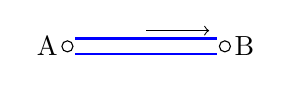
\begin{tikzpicture}
\draw (0,0) circle (2pt) node[left] {A};
\draw (2,0) circle (2pt) node[right] {B};
\draw[blue,thick] (0.1,0.1) -- (1.9,0.1);
\draw[blue,thick] (0.1,-0.1) -- (1.9,-0.1);
\draw[->] (1,0.2) -- (1.8,0.2);
\end{tikzpicture}
\caption{Feromon izleri ve yol seçimi}
\label{fig:aco_path}
\end{marginfigure}

\subsection{Diferansiyel Evrim (DE) Algoritması}
Vektör tabanlı evrimsel bir optimizasyon algoritmasıdır. Sürekli optimizasyon problemlerinde etkili sonuçlar verir.

\subsubsection{Temel Operatörler}
\begin{itemize}
    \item Mutasyon vektörü
    \item Çaprazlama
    \item Seçim
    \item Ölçekleme faktörü (F)
    \item Çaprazlama oranı (CR)
\end{itemize}

\begin{equation}
v_i = x_{r1} + F(x_{r2} - x_{r3})
\end{equation}

\begin{tcolorbox}[title=DE Stratejileri]
\begin{itemize}
    \item DE/rand/1/bin
    \item DE/best/1/bin
    \item DE/rand/2/bin
    \item DE/best/2/bin
    \item DE/current-to-best/1/bin
\end{itemize}
\end{tcolorbox}

\subsubsection{Algoritmanın Adımları}
\begin{enumerate}
    \item Başlangıç popülasyonunu oluştur
    \item Her nesilde:
        \begin{itemize}
            \item Mutasyon vektörlerini üret
            \item Çaprazlama uygula
            \item Seçim yap
        \end{itemize}
    \item Durma kriteri sağlanana kadar devam et
\end{enumerate}

\sidenote{Diferansiyel evrim algoritması, sürekli optimizasyon problemlerinde özellikle etkilidir. Parametre ayarı görece kolaydır ve yakınsama hızı yüksektir.}

\subsection{Yapay Arı Kolonisi (ABC) Optimizasyonu}
Bal arılarının yiyecek arama davranışından esinlenen bir optimizasyon algoritmasıdır.

\subsubsection{Arı Tipleri ve Görevleri}
\begin{itemize}
    \item İşçi arılar: Mevcut kaynakların araştırılması
    \item Gözcü arılar: Umut verici kaynakların değerlendirilmesi
    \item Kâşif arılar: Yeni kaynakların keşfi
\end{itemize}

\begin{equation}
v_{ij} = x_{ij} + \phi_{ij}(x_{ij} - x_{kj})
\end{equation}

\begin{marginfigure}
\centering
\begin{tikzpicture}
\draw[->] (0,0) -- (4,0) node[right] {$x$};
\draw[->] (0,0) -- (0,4) node[above] {$f(x)$};
\filldraw[blue] (1,2) circle (2pt) node[above] {İşçi};
\filldraw[red] (2,3) circle (2pt) node[above] {Gözcü};
\filldraw[green] (3,1) circle (2pt) node[above] {Kâşif};
\end{tikzpicture}
\caption{ABC'de farklı arı tiplerinin rolü}
\label{fig:abc_bees}
\end{marginfigure}

\subsubsection{Algoritmanın Adımları}
\begin{enumerate}
    \item Başlangıç besin kaynaklarını belirle
    \item Her döngüde:
        \begin{itemize}
            \item İşçi arı fazı
            \item Gözcü arı fazı
            \item Kâşif arı fazı
        \end{itemize}
    \item Durma kriteri sağlanana kadar devam et
\end{enumerate}

\subsection{Kuantum ve Hibrit Optimizasyon Algoritmaları}
Kuantum mekaniği prensiplerinden esinlenen ve farklı algoritmaların güçlü yönlerini birleştiren yaklaşımlar.

\subsubsection{Kuantum-Esinli Algoritmalar}
\begin{itemize}
    \item Kuantum parçacık sürüsü
    \item Kuantum genetik algoritma
    \item Kuantum tavlama benzetimi
\end{itemize}

\begin{equation}
\psi(x,t) = \frac{1}{\sqrt{2\pi\sigma^2}} e^{-\frac{(x-\mu)^2}{2\sigma^2}}
\end{equation}

\begin{tcolorbox}[title=Kuantum Mekanizmasının Avantajları]
\begin{itemize}
    \item Daha iyi keşif yeteneği
    \item Lokal optimumlardan kaçınma
    \item Hızlı yakınsama
    \item Belirsizlik prensibinden faydalanma
\end{itemize}
\end{tcolorbox}

\subsection{Diğer Metasezgisel Optimizasyon Algoritmaları}
Akademik literatüre her yıl onlarca yeni metasezgisel optimizasyon algoritması eklenmektedir. Bu algoritmaların, bazıları hala oldukça özgün yaklaşımlar ortaya koyabimektedir. Ancak temel sınıflandırmalar dahilinde birçoğu daha önceki algoritmaların belli mekanizmalarını belli ölçüde taklit ederek geliştirmektedir. Bu konuya akademik perspektifin dışından bakan bir mühendis için bazı temel algoritmaları anlamak ve uygulayabilmek yeni algoritmaları sürekli olarak takip etmekten çok daha faydalıdır. Özellikle yapay zekanın gelişimi de düşünüldüğünde esas önemli olan doğru pratik sahalarında teorik bilgiyi hayata geçirmetir.

